\chapter{Categorical organisation of the ornament--refinement framework}
\label{chap:categorical}

\section{Formalisation of categories}
\label{sec:categories}

In this section we formalise some basic category-theoretic terms in Agda, establishing vocabulary for Sections \ref{sec:organisation}~and~\ref{sec:isomorphisms}.

\subsection{Definitions of categories and functors}

We will define a category to be a set of objects and sets of morphisms indexed by source and target, together with the usual laws.
Special attention must be paid to equality on morphisms, though, which is usually coarser than definitional equality --- for example, in the category of sets and (total) functions, it is necessary to identify functions up to extensional equality, so uniqueness of morphisms in universal properties would make sense.
One simple way to achieve this in Agda's intensional setting is to use \emph{setoids}~\cite{Barthe-setoids} --- i.e., sets with an explicitly specified equivalence relation --- to represent sets of morphisms.
Subsequently, all operations on morphisms should respect the equivalence.

In Agda, the type of setoids can be defined as a record which contains a carrier set, an equivalence relation on the set, and the three laws for the equivalence relation:%
\footnote{The definition of setoids uses Agda's universe polymorphism, so the definition can be instantiated at suitable levels of the |Set| hierarchy as needed.
We will give the first few universe-polymorphic definitions with full detail about the levels, but will later switch to writing just `|Set _|' to suppress the noise.}
\begin{code}
record Setoid {c d : Level} : Set (suc (c ⊔ d)) where
  field
    Carrier  :  Set c
    _≈_      :  Carrier → Carrier → Set d
    refl'    :  ∀ {x} → x ≈ x
    sym      :  ∀ {x y} → x ≈ y → y ≈ x
    trans    :  ∀ {x y z} → x ≈ y → y ≈ z → x ≈ z
\end{code}
For example, we can define a setoid of functions that uses extensional equality:
\begin{code}
FunSetoid : Set → Set → Setoid
FunSetoid A B = record  {    Carrier  =  A → B
                        sep  _≈_      =  _≐_
                        sep  proofs-of-laws  }
\end{code}
where |_≐_| is defined by |f ≐ g = ∀ x → f x ≡ g x|.
Proofs of the three laws are omitted from the paper.

\begin{figure}
\begin{code}
record Category {l m n : Level} : Set (suc (l ⊔ m ⊔ n)) where
  field
    Object    :  Set l
    Morphism  :  Object → Object → Setoid {m} {n}

  _==>_ : Object → Object → Set m
  X ==> Y = Setoid.Carrier (Morphism X Y)
  _≈_ : ∀ {X Y} → X ==> Y → X ==> Y → Set n
  _≈_ {X} {Y} = Setoid._≈_ (Morphism X Y)

  field
    _·_  :   ∀ {X Y Z} → Y ==> Z → X ==> Y → X ==> Z
    id   :   ∀ {X} → X ==> X
    id-l    :  ∀ {X Y} (f : X ==> Y) → id · f ≈ f
    id-r    :  ∀ {X Y} (f : X ==> Y) → f · id ≈ f
    assoc   :  ∀ {X Y Z W}
               (f : Z ==> W) (g : Y ==> Z) (h : X ==> Y) →
               (f · g) · h ≈ f · (g · h)
    cong-l  :  ∀ {X Y Z} {f g : Y ==> Z} (h : X ==> Y) →
               f ≈ g → f · h ≈ g · h
    cong-r  :  ∀ {X Y Z} (h : Y ==> Z) {f g : X ==> Y} →
               f ≈ g → h · f ≈ h · g
\end{code}
\caption{Definition of categories.}
\label{fig:category}
\end{figure}

Similarly, we can define the type of categories as a record containing a set of objects, a collection of setoids of morphisms indexed by source and target (so morphisms with the same source and target --- and only such morphisms --- can be compared for equality), the composition operator on morphisms, the identity morphisms, and the laws of categories.
The definition is shown in \autoref{fig:category}.
Two notations are introduced to improve readability: |X ==> Y| is defined to be the carrier set of the setoid of morphisms from~|X| to~|Y|, and |f ≈ g| is defined to be the equivalence between the morphisms |f|~and~|g| as specified by the setoid to which |f|~and~|g| belong.
The last two laws |cong-l| and |cong-r| require composition of morphisms to respect the equivalence on morphisms; they are given in this form to work better with the equational reasoning combinators commonly used in Agda (see, for example, the AoPA library~\cite{Mu-AoPA}).
Now we can define the category |Fun| of sets and (total) functions as
\begin{code}
Fun : Category
Fun = record  {    Object    =  Set
              sep  Morphism  =  FunSetoid
              sep  _·_  =  _∘_
              sep  id   =  (lambda(x)) x
              sep  proofs-of-laws }
\end{code}
Another important category that we will make use of is |Fam|, the category of families of sets and families of functions, which is useful for talking about componentwise structures.
An object in |Fam| has type |(Σ'(I ∶ Set)) I → Set|, i.e., it is a set~|I| and a family of sets indexed by~|I|;
a morphism from |(J , Y)| to |(I , X)| is a function |e : J → I| and a family of functions from |Y j| to |X (e j)| for each |j : J|.
\begin{code}
Fam : Category
Fam = record
  {    Object    = (Σ'(I ∶ Set)) I → Set
  sep  Morphism  =
         (lambda((J , Y) (I , X))) record
           {    Carrier  =  (Σ'(e ∶ J → I)) Y ⇉ (X ∘ e)
           sep  _≈_      =  (lambda((e , u) (e' , u')))
                              (e ≐ e') × (∀ {j} → u {j} JMEq' u' {j})
           sep  proofs-of-laws }
  sep  _·_  = (lambda((e , u) (f , v))) (e ∘ f) , ((lambda({k})) u {f k} ∘ v {k})
  sep  id   =  ((lambda(x)) x) , ((lambda({i} x)) x)
  sep  proofs-of-laws }
\end{code}
Note that the equivalence on morphisms is defined to be componentwise extensional equality, which is formulated with the help of McBride's ``John Major'' heterogeneous equality |_JMEq_|~\cite{McBride-thesis} --- the equivalence |_JMEq'_| is defined by |g JMEq' h = ∀ x → g x JMEq h x|.
(Given |y : Y j| for some |j : J|, the types of |u {j} y| and |u' {j} y| are not definitionally equal but only provably equal, so it is necessary to employ heterogeneous equality.)

\begin{figure}
\begin{code}
record Functor
  {l m n l' m' n' : Level}
  (C : Category {l} {m} {n}) (D : Category {l'} {m'} {n'}) :
  Set (l ⊔ m ⊔ n ⊔ l' ⊔ m' ⊔ n') where
  field
    object    :  CObject → DObject
    morphism  :  ∀ {X Y} → X =C=> Y → object X =D=> object Y
    ≈-respecting :
      ∀ {X Y} {f g : X =C=> Y} →
      f ≈C g → morphism f ≈D morphism g
    id-preserving :
      ∀ {X} → morphism (idC {X}) ≈D idD {object X}
    comp-preserving :
      ∀ {X Y Z} (f : Y =C=> Z) (g : X =C=> Y) →
      morphism (f ·C g) ≈D (morphism f ·D morphism g)
\end{code}
\caption{Definition of functors.}
\label{fig:functor}
\end{figure}

We will also need functors, whose definition is shown in \autoref{fig:functor}: a functor consists of two mappings, one on objects and the other on morphisms, where the morphism part respects equivalence on morphisms and preserves identity and composition.
For example, we have two forgetful functors from |Fam| to |Fun|, one summing components together
\begin{code}
FamF : Functor Fam Fun
FamF = record  {    object    =  (lambda((I  ,  X  )))  Σ I X
               sep  morphism  =  (lambda((e  ,  u  )))  e ** u
               sep  proofs-of-laws }
\end{code}
%|FamF| gives one interpretation of |Fam| (in |Fun|):
%In |Fam|, an object |(I , X)| is canonically understood as |Σ I X|, but the index set and the component sets are kept separate.
%A morphism in |Fam| exploits such separation and consists of a function~|e| on the index sets and a family~|u| of functions only between the corresponding components as specified by~|e|, so computation on the indices can always be carried out independently.
%(This is witnessed by the existence of another forgetful functor from |Fam| to |Fun| whose object and morphism parts are both |proj₁|.)
%Functions on sums of indexed sets that can be described in |Fam| are thus very well-behaved, in the sense that when a function |e ** u : Σ J Y → Σ I X| is applied to some |(j , y)|, without inspecting~|y| we can already determine that the result would have index~|e j| --- this cannot be said about an arbitrary function of type |Σ J Y → Σ I X|.
and the other extracting the index part.
\begin{code}
FamI : Functor Fam Fun
FamI = record  {    object    =  (lambda((I  ,  X  )))  I
               sep  morphism  =  (lambda((e  ,  u  )))  e
               sep  proofs-of-laws }
\end{code}
The functor laws should be proved for both functors alongside their object and morphism maps.
In particular, we need to prove that the morphism part respects equivalence: for |FamF| this means we need to prove, for all |e : J → I|, |u : Y ⇉ (X ∘ e)|, |f : J → I|, and |v : Y ⇉ (X ∘ f)|, that
\[ |(e ≐ f) × (∀ {j} → u {j} JMEq' v {j}) → (e ** u ≐ f ** v)| \]
and for |FamI| we need to prove
\[ |(e ≐ f) × (∀ {j} → u {j} JMEq' v {j}) → (e ≐ f)| \]
both of which can be easily discharged.

\subsection{Definition of pullbacks}

We will define a pullback to be a product in the suitable slice category, where a product is defined to be a terminal object in the suitable span category.
Below we give definitions of all these terms in logical order.
Let |C : Category| in what follows.

\begin{figure}[t]
\begin{code}
record Slice C B : Set _ where
  constructor slice
  field
    T  :  Object
    s  :  T ==> B

record SliceMorphism C B (s t : Slice C B) : Set _ where
  constructor sliceMorphism
  field
    m : Slice.T s ==> Slice.T t
    triangle  :  Slice.s t · m ≈ Slice.s s

SliceCategory C B : Category
SliceCategory C B =
  record
    {    Object    =  Slice C B
    sep  Morphism  =
           (lambda(s t))  record
                            {    Carrier = SliceMorphism C B s t
                            sep  _≈_ = (lambda(f g))  SliceMorphism.m f ≈
                                                      SliceMorphism.m g
                            sep proofs-of-laws }
    sep  proofs-of-laws }

record Span C L R : Set _ where
  constructor span
  field
    M  :  Object
    l  :  M ==> L
    r  :  M ==> R

record SpanMorphism C L R (s t : Span C L R) : Set _ where
  constructor spanMorphism
  field
    m : Span.M s ==> Span.M t
    triangle-l  :  Span.l  t · m ≈ Span.l  s
    triangle-r  :  Span.r  t · m ≈ Span.r  s

SpanCategory C L R : Category
SpanCategory C L R =
  record
    {    Object    =  Span C L R
    sep  Morphism  =
           (lambda(s t))  record
                            {    Carrier = SpanMorphism C L R s t
                            sep  _≈_ = (lambda(f g))  SpanMorphism.m f ≈
                                                      SpanMorphism.m g
                            sep proofs-of-laws }
    sep  proofs-of-laws }
\end{code}
\caption{Definitions of slice categories and span categories, where |C : Category| and |B|, |L|, |R| are objects of~|C|.}
\label{fig:slice-and-span}
\end{figure}

\begin{itemize}[leftmargin=*]

\item A \emph{slice category} based on~|C| is parametrised by an object~|B|; its objects are those morphisms in~|C| with target~|B| and its morphisms are mediating morphisms giving rise to commutative triangles --- diagrammatically,
\[ \text{objects }
\begin{tikzpicture}[baseline=(s.base)]
\matrix (m) [matrix of math nodes, row sep=4ex]
{ T \\
  B \\ };
\path[->]
(m-1-1) edge node[left](s){$s$} (m-2-1);
\end{tikzpicture}
\qquad\text{and}\qquad\text{morphisms }
\begin{tikzpicture}[baseline=(s.base)]
\matrix (m) [matrix of math nodes, row sep=5ex, column sep=.4em]
{ T &   & T\smash{'} \\
    & B & \\ };
\path[->]
(m-1-1) edge node[left](s){$s$} (m-2-2)
(m-1-3) edge node[right]{$s\smash{'}$} (m-2-2)
(m-1-1) edge node[above]{$m$} (m-1-3);
\end{tikzpicture} \]
The slice objects and morphisms are defined in Agda as two records; they are shown in the upper half of \autoref{fig:slice-and-span} along with the definition of slice categories.
Note that the equivalence on slice morphisms is defined as only the equivalence on the mediating morphisms, essentially achieving proof-irrelevance.

\item \emph{Span categories} are similar: parametrised by two objects |L|~and~|R|, a span category has
\[ \text{objects }
\begin{tikzpicture}[baseline=(m-1-1.base)]
\matrix (m) [matrix of math nodes, column sep=1.2em]
{ L & M & R \\ };
\path[->]
(m-1-2) edge node[above]{$l$} (m-1-1)
(m-1-2) edge node[above]{$r$} (m-1-3);
\end{tikzpicture}
\quad\text{and}\quad \text{morphisms }
\begin{tikzpicture}[baseline=(m-2-1.base)]
\matrix (m) [matrix of math nodes, row sep=.6ex, column sep=1.2em]
{   & M           & \\
  L &             & R \\
    & M\rlap{$'$} & \\ };
\path[->]
(m-1-2) edge node[above]{$l$} (m-2-1)
(m-1-2) edge node[above]{$r$} (m-2-3)
(m-3-2) edge node[below]{$l$\rlap{$'$}} (m-2-1)
(m-3-2) edge node[below]{$r$\rlap{$'$}} (m-2-3)
(m-1-2) edge node[left]{$m$} (m-3-2);
\end{tikzpicture} \]
The Agda definitions are shown in the lower half of \autoref{fig:slice-and-span}, and are similar to those for slice categories.

\item An object~|X| in~|C| is \emph{terminal} if it satisfies the universal property that for every object~|Y| there is a unique morphism from~|Y| to~|X|:
\begin{code}
Terminal C : Object → Set _
Terminal C X =
  (Y : Object) → (Σ'(f ∶ Y ==> X)) Unique (Morphism Y X) f
\end{code}
where uniqueness is defined relative to a setoid:
\begin{code}
Unique : (S : Setoid) → Carrier_S → Set _
Unique S x = (y : Carrier_S) → x ≈S y
\end{code}

\item A \emph{product} of two objects |X|~and~|Y| in~|C| is then a |Span C X Y| that is terminal in |SpanCategory C X Y|:
\begin{code}
Product C X Y : Span C X Y → Set _
Product C X Y = Terminal (SpanCategory C X Y)
\end{code}

\item A \emph{pullback} of two slices |f|, |g : Slice C X| is a product of |f|~and~|g| in |SliceCategory C X|:
Define the type of \emph{squares} based on |f|~and~|g| as
\begin{code}
Square C f g : Set _
Square C f g = Span (SliceCategory C X) f g
\end{code}
or diagrammatically,
\[ 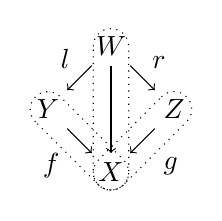
\begin{tikzpicture}[scale=.8, baseline=(Y.base)]
\node(X) at (0, 0) {$X$};
\node(Y) at (-1, 1) {$Y$};
\node(Z) at (1, 1) {$Z$};
\node(W) at (0, 2) {$W$};
\path[->]
(W) edge node[above left]{$l$} (Y)
(W) edge node[above right]{$r$} (Z)
(W) edge (X)
(Y) edge (X)
(Z) edge (X);
\draw[dotted] ([xshift=-5.658pt,yshift=-5.658pt]Y.center) arc (225:45:8pt) -- ([xshift=5.658pt,yshift=5.658pt]X.center) arc (45:-135:8pt) -- cycle;
\draw[dotted] ([xshift=-8pt]W.center) arc (180:0:8pt) -- ([xshift=8pt]X.center) arc (0:-180:8pt) -- cycle;
\draw[dotted] ([xshift=-5.658pt,yshift=5.658pt]Z.center) arc (135:-45:8pt) -- ([xshift=5.658pt,yshift=-5.658pt]X.center) arc (-45:-225:8pt) -- cycle;
\node at (-.95, .1) {$f$};
\node at (.95, .1) {$g$};
\end{tikzpicture}
\quad\text{which is the same as}\quad
\begin{tikzpicture}[scale=.8, baseline=($(W)!.5!(X)$)]
\node(X) at (0, 0) {$X$};
\node(XL) at (-1.25, 0) {$X$};
\node(XR) at (1.25, 0) {$X$};
\node(Y) at (-1.25, 1.25) {$Y$};
\node(Z) at (1.25, 1.25) {$Z$};
\node(W) at (0, 1.25) {$W$};
\node at ([yshift=-1pt]$(XL)!.5!(X)$) {$=$};
\node at ([yshift=-1pt]$(X)!.5!(XR)$) {$=$};
\path[->]
(W) edge node[above]{$l$} (Y)
(W) edge node[above]{$r$} (Z)
(W) edge (X)
(Y) edge (XL)
(Z) edge (XR);
\draw[dotted] ([xshift=-8pt]W.center) arc (180:0:8pt) -- ([xshift=8pt]X.center) arc (0:-180:8pt) -- cycle;
\draw[dotted] ([xshift=-8pt]Y.center) arc (180:0:8pt) -- ([xshift=8pt]XL.center) arc (0:-180:8pt) -- cycle;
\draw[dotted] ([xshift=-8pt]Z.center) arc (180:0:8pt) -- ([xshift=8pt]XR.center) arc (0:-180:8pt) -- cycle;
\node at (-1.25, 1.8) {$f$};
\node at (1.25, 1.8) {$g$};
\end{tikzpicture} \]
In a square~|q|, we will refer to the object |Slice.T (Span.M q)|, i.e., the node~|W| in the diagrams above, as the \emph{vertex} of~|q|.
A pullback of |f|~and~|g| is then a square based on |f|~and~|g| that satisfies
\begin{code}
Pullback C f g : Square C f g → Set _
Pullback C f g = Product (SliceCategory C X) f g
\end{code}
Equivalently, if we define the \emph{square category} based on |f|~and~|g| as
\begin{code}
SquareCategory C f g : Category
SquareCategory C f g =
  SpanCategory (SliceCategory C X) f g
\end{code}
then a pullback of |f|~and~|g| is a terminal object in the square category based on |f|~and~|g| --- indeed, |Product (SliceCategory C X) f g| is definitionally equal to |Terminal (SquareCategory C f g)|.

\end{itemize}

The most important category-theoretic fact that we will use in this paper is that the vertices of any two pullbacks of the same slices are isomorphic.
Define the type of isomorphisms between two objects |X|~and~|Y| in~|C| as
\begin{code}
record Iso C X Y : Set _ where
  field
    to    :  X ==> Y
    from  :  Y ==> X
    from-to-inverse  :  from · to ≈ id
    to-from-inverse  :  to · from ≈ id
\end{code}
(The isomorphism relation |_≅_| we used in \autoref{sec:ornaments} is formally defined as |Iso Fun|.)
Then we can formulate the following lemma:
If |p|, |q : Square C f g| are both pullbacks, then we have an isomorphism
\[ |Iso C (Slice.T (Span.M p)) (Slice.T (Span.M q))| \]

\section{Categorical organisation of the ornament--refinement framework}
\label{sec:organisation}

\begin{figure*}
\begin{center}
\begin{tikzpicture}
\matrix (m) [matrix of math nodes, column sep=.5em, nodes={anchor=west}]
{        & |Ōrn|                       & |FRef|                          & |Fam|                           & |Fun| \\[6ex]
|Object| & |(Σ'(I ∶ Set)) Desc I|      & |(Σ'(I ∶ Set)) I → Set|         & |(Σ'(I ∶ Set)) I → Set|         & |Set| \\[.5ex]
|_==>_|  & |(lambda((J , E) (I , D))|  & |(lambda((J , Y) (I , X)))|     & |(lambda((J , Y) (I , X)))|     & |(lambda(A B)) A → B| \\[-1.2ex]
         & \kern.74em|(Σ'(e ∶ J → I)) Orn e D E| & \kern.74em|(Σ'(e ∶ J → I)) FRefinement e X Y| & \kern.74em|(Σ'(e ∶ J → I)) Y ⇉ (X ∘ e)| \\ };
\path[->]
(m-1-2) edge[bend right] node[above]{|RSem|} (m-1-3)
(m-1-2) edge[bend left] node[above]{|Ind|} (m-1-4.north)
(m-1-3) edge[bend left] node[below]{|FRefF|} (m-1-4)
(m-1-4) edge[bend left] node[above]{|FRefC|} (m-1-3)
(m-1-4) edge[bend left] node[above]{|FamF|} (m-1-5)
(m-1-4) edge[bend right] node[above]{|FamI|} (m-1-5);
\end{tikzpicture}
\end{center}
\caption{Categories (whose sets of objects and morphisms are listed below) and functors for the ornament--refinement framework.}
\label{fig:categories}
\end{figure*}

We proceed to organise the ornament--refinement framework under several concrete categories and functors, aiming to clarify the overall structure of the framework, and then derive useful pullback properties from parallel composition of ornaments.

\subsection{The category of type families and refinement families}
\label{sec:FRef}

We will see that the category |FRef| of type families and refinement families has a very close relationship to the category |Fam|.
An object in |FRef| is an indexed family of sets as in |Fam|, and a morphism from |(J , Y)| to |(I , X)| consists of a function |e : J → I| on the indices and a refinement family of type |FRefinement e X Y|.
As for the equivalence on morphisms, it suffices to use extensional equality on the index functions and componentwise equivalence on refinement families, where the equivalence on refinements is defined to be extensional equality on their forgetful functions (extracted by |Refinement.forget|).
In Agda:
\begin{code}
FRef : Category
FRef = record
  {    Object    =   (Σ'(I ∶ Set)) I → Set
  sep  Morphism  =
         (lambda((J , Y) (I , X))) record
           {    Carrier  =   (Σ'(e ∶ J → I)) FRefinement e X Y
           sep  _≈_      =
                  (lambda((e , rs) (e' , rs')))
                    (e ≐ e') ×
                    (∀ j →  Refinement.forget (rs   (ok j)) JMEq'
                            Refinement.forget (rs'  (ok j)))
           sep  proofs-of-laws }
  sep  proofs-of-laws }
\end{code}
Two facts support our choice of refinement equivalence: (i)~under this definition, if two refinements are equivalent, then their promotion predicates are pointwise isomorphic, i.e., we have
\begin{code}
forget-iso :
  {X Y : Set} (r s : Refinement X Y) →
  (Refinement.forget r ≐ Refinement.forget s) →
  ∀ x → Refinement.P r x ≅ Refinement.P s x
\end{code}
and (ii)~we get a forgetful functor |FRefF : Functor FRef Fam| which is identity on objects and componentwise |Refinement.forget| on morphisms, the latter respecting equivalence automatically.
\begin{code}
FRefF : Functor FRef Fam
FRefF = record
  {    object     =  (lambda((I , X))) I , X
  sep  morphism   =
         (lambda((e , rs))) e , ((lambda({j})) Refinement.forget (rs (ok j)))
  sep  proofs-of-laws }
\end{code}
Note that a refinement family from |X : I → Set| to |Y : J → Set| is deliberately cast as a morphism in the opposite direction from |(J , Y)| to |(I , X)|, so |FRefF| remains a familiar covariant functor rather than a contravariant one.
Think of this as suggesting the direction of the forgetful functions of refinements.

The above discussion suggests that the essential ingredient of a refinement is just its forgetful function.
Indeed, from any function we can construct a \emph{canonical refinement}:
\begin{code}
canonRef : {X Y : Set} → (Y → X) → Refinement X Y
canonRef {X} {Y} f = record
  {    P  =  (lambda(x)) (Σ'(y ∶ Y)) f y ≡ x
  sep  i  =  record  {    to    =  (split(f)(split(((lambda(y)) y))((lambda(y) refl))))
                     sep  from  =  proj₁ ∘ proj₂
                     sep  proofs-of-laws } }
\end{code}
(The operator |split-op| is defined by |(split(g)(h)) = (lambda(x)) (g x , h x)|.)
The canonical promotion predicate is very simplistic: to promote some |x : X| to type~|Y|, we are required to supply a complete |y : Y| such that |x|~can be recovered from~|y| (rather than only the necessary information that augments~|x| to an element of~|Y|).
Any refinement |r : Refinement X Y| is equivalent to |canonRef (Refinement.forget r)|, so by |forget-iso| we have
\[ |Refinement.P r x| ~\cong~ |(Σ'(y ∶ Y)) Refinement.forget r y ≡ x| \]
for all |x : X|.
That is, a promotion predicate is always pointwise isomorphic to the canonical promotion predicate.
Thus all the refinement mechanism provides is a convenient way of expressing intensional (representational) optimisations of the canonical promotion predicate --- extensionally, |FRef| is no more powerful than |Fam|.
This is reflected in the existence of a functor |FRefC : Functor Fam FRef|, whose object part is identity and whose morphism part is componentwise |canonRef|:
\begin{code}
FRefC : Functor Fam FRef
FRefC = record
  {    object    =  (lambda((I , X  ))) I , X
  sep  morphism  =  (lambda((e , u  ))) e , ((lambda((ok j))) canonRef (u {j}))
  sep  proofs-of-laws }
\end{code}
|FRefC| is strictly inverse to |FRefF|, forming an isomorphism (not merely an equivalence) of categories between |FRef| and |Fam|.

\subsection{The category of descriptions and ornaments}
\label{sec:Orn}

The category |Ōrn| has objects of type |(Σ'(I ∶ Set)) Desc I|, i.e., descriptions paired with index sets, and morphisms from |(J , E)| to |(I , D)| of type |(Σ'(e ∶ J → I)) Orn e D E|, i.e., ornaments paired with index erasure functions.
We also need to devise an equivalence on ornaments
\begin{code}
OrnEq :
  {I J : Set} {e e' : J → I} {D : Desc I} {E : Desc J} →
  Orn e D E → Orn e' D E → Set
\end{code}
such that it implies extensional equality of |e|~and~|e'| and that of ornamental forgetful functions:
\begin{code}
OrnEq-forget :
  {I J : Set} {e e' : J → I} {D : Desc I} {E : Desc J}
  (O : Orn e D E) (P : Orn e' D E) → OrnEq O P →
  (e ≐ e') × (∀ {j} → forget O {j} JMEq' forget P {j})
\end{code}
We omit the detail of |OrnEq| from the paper (which depends on the detail of the universe of ornaments).
Morphism composition is sequential composition, and there is a family of \emph{identity ornaments}
\[ |idOrn : {I : Set} {D : Desc I} → Orn ((lambda(i)) i) D D| \]
such that |idOrn {I} {D}| simply expresses that |D| is identical to itself.
Unsurprisingly, the identity ornaments serve as identity of sequential composition.
To summarise:
\begin{code}
Ōrn : Category
Ōrn = record
  {    Object    =  (Σ'(I ∶ Set)) Desc I
  sep  Morphism  =
         (lambda((J , E) (I , D))) record
           {    Carrier  =  (Σ'(e ∶ J → I)) Orn e D E
           sep  _≈_      =  (lambda((e , O) (e' , O'))) OrnEq O O'
           sep  proofs-of-laws }
  sep  _·_  =  (lambda ((e , O) (f , P))) (e ∘ f) , (O ⊙ P)
  sep  id   =  ((lambda(i)) i) , idOrn
  sep  proofs-of-laws }
\end{code}
A functor |Ind : Functor Ōrn Fam| can then be constructed, which gives the ordinary semantics of descriptions and ornaments: the object part of |Ind| decodes a description |(I , D)| to its least fixed point |(I , μ D)|, and the morphism part translates an ornament |(e , O)| to the forgetful function |(e , forget O)|, the latter respecting equivalence by virtue of |OrnEq-forget|.
\begin{code}
Ind : Functor Ōrn Fam
Ind = record  {    object    =  (lambda((I , D  ))) I , μ D
              sep  morphism  =  (lambda((e , O  ))) e , forget O
              sep  proofs-of-laws }
\end{code}

\subsection{Pullback properties for parallel composition}
\label{sec:pullback-properties}

We are now ready to state the pullback properties for parallel composition of ornaments.
With suitable choices of encoding for the universes, we could attempt to establish that, for any two ornaments |O : Orn e D E| and |P : Orn f D F| where |D : Desc I|, |E : Desc J|, and |F : Desc K|, the following square in |Ōrn| is a pullback:
\begin{center}
\begin{tikzpicture}[scale=3]
\node(D) at (1, 0) {|I , D|};
\node(E) at (0, 0) {|J , E|};
\node(F) at (1, .5) {|K , F|};
\node(P) at (0, .5) {|e ⋈ f , ⌊ O ⊗ P ⌋|};
\path[->, font=\scriptsize]
(E) edge node[below]{|e , O|} (D)
(F) edge node[right]{|f , P|} (D)
(P) edge node{\labelonarrow{|pull, ⌈ O ⊗ P ⌉|}} (D)
(P) edge node[left]{\llap{|π₁ , diffOrn-l O P|}} (E)
(P) edge node[above,yshift=.5ex]{|π₂ , diffOrn-r O P|} (F);
\end{tikzpicture}
\end{center}
This square is encoded in Agda as
\begin{code}
pc-square : Square Ōrn (slice (J , E) (e , O)) (slice (K , F) (f , P))
pc-square = span  (slice (e ⋈ f , ⌊ O ⊗ P ⌋) (pull, ⌈ O ⊗ P ⌉))
                  (sliceMorphism (π₁  , diffOrn-l  O P)  (hole()(1)))
                  (sliceMorphism (π₂  , diffOrn-r  O P)  (hole()(2)))
\end{code}
where goal~1 has type |OrnEq (O ⊙ diffOrn-l O P) ⌈ O ⊗ P ⌉| and goal~2 has type |OrnEq (P ⊙ diffOrn-r O P) ⌈ O ⊗ P ⌉|, both of which can be discharged.%
\footnote{Since the structure of Agda terms like |pc-square| can be reconstructed from commutative diagrams and the categorical definitions, in the rest of the paper we will present only the commutative diagrams and omit the underlying Agda terms.}
The pullback property of |pc-square|, i.e., |Pullback Ōrn _ _ pc-square|, is not too useful by itself, though: |Ōrn| is quite a restricted category, so a universal property established in |Ōrn| has limited applicability.
Instead, we are more interested in the pullback property of the image of the above square under |Ind| in |Fam|, which is stated in the follow theorem.
If |O : Orn e D E| and |P : Orn f D F| where |D : Desc I|, |E : Desc J|, and |F : Desc K|, then the following square in |Fam| is a pullback.
\begin{center}
\begin{tikzpicture}[scale=3]
\node(D) at (1, 0) {|I , μ D|};
\node(E) at (0, 0) {|J , μ E|};
\node(F) at (1, .5) {|K , μ F|};
\node(P) at (0, .5) {|e ⋈ f , μ ⌊ O ⊗ P ⌋|};
\draw[very thick] (.05, .32) -- (.15, .32) -- (.15, .42);
\path[->, font=\scriptsize]
(E) edge node[below]{|e , forget O|} (D)
(F) edge node[right]{\rlap{|f , forget P|}} (D)
(P) edge node{\labelonarrow{|pull, forget ⌈ O ⊗ P ⌉|}} (D)
(P) edge node[left]{\llap{|π₁ , forget (diffOrn-l O P)|}} (E)
(P) edge node[above,yshift=1ex]{|π₂ , forget (diffOrn-r O P)|} (F);
\end{tikzpicture}
\end{center}
\noindent The proof of the universal property boils down to, very roughly speaking, construction of an inverse to
\[ |(split(forget (diffOrn-l O P))(forget (diffOrn-r O P)))| \]
which involves tricky manipulation of equality proofs but is achievable.
% \jg{``involves tedious but straightforward manipulation of equality proofs''?} \note{Urr, it is really tricky. I wouldn't describe it as straightforward, as it almost broke my head.}
After the pullback property is established in |Fam|, since |FamF| is pullback-preserving, we also get a pullback square in |Fun|.
If |O : Orn e D E| and |P : Orn f D F| where |D : Desc I|, |E : Desc J|, and |F : Desc K|, then the following square in |Fun| is a pullback.
\begin{center}
\begin{tikzpicture}[scale=3]
\node(D) at (1, 0) {|Σ I (μ D)|};
\node(E) at (0, 0) {|Σ J (μ E)|};
\node(F) at (1, .5) {|Σ K (μ F)|};
\node(P) at (0, .5) {|Σ (e ⋈ f) (μ ⌊ O ⊗ P ⌋)|};
\draw[very thick] (.05, .32) -- (.15, .32) -- (.15, .42);
\path[->, font=\scriptsize]
(E) edge node[below]{|e ** forget O|} (D)
(F) edge node[right]{\rlap{|f ** forget P|}} (D)
(P) edge node{\labelonarrow{|pull ** forget ⌈ O ⊗ P ⌉|}} (D)
(P) edge node[left]{\llap{|π₁ ** forget (diffOrn-l O P)|}} (E)
(P) edge node[above,yshift=1ex]{|π₂ ** forget (diffOrn-r O P)|} (F);
\end{tikzpicture}
\end{center}

To translate |Ōrn| to |FRef|, i.e., datatype declarations to refinements, a naive way is to use the composite functor
\[ \begin{tikzpicture}
\matrix (m) [matrix of math nodes, column sep=4em]
{ \smash{|Ōrn|}\vphantom{|Fam|} & |Fam| & |FRef| \\ };
\path[->]
(m-1-1) edge node[above]{|Ind|} (m-1-2)
(m-1-2) edge node[above]{|FRefC|} (m-1-3);
\end{tikzpicture} \]
The resulting refinements would then use canonical promotion predicates.
However, the whole point of incorporating |Ōrn| in the framework is that we can construct an alternative functor |RSem| directly from |Ōrn| to |FRef|.
The functor |RSem| is extensionally equal to the above composite functor, but intensionally very different.
Its object part still takes the least fixed point of a description, but its morphism part is the refinement semantics of ornaments given in \autoref{sec:refinements}, whose promotion predicates have a more efficient representation.
\begin{code}
RSem : Functor Ōrn FRef
RSem = record
  {    object    =  (lambda((I , D))) I , μ D
  sep  morphism  =
         (lambda((e , O))) e , (  (lambda((ok j))) record  {    P  =  OptP O (ok j)
                                                           sep  i  =  (hole()(3)) })
  sep  proofs-of-laws }
\end{code}
We will give goal~3, i.e., the ornamental promotion isomorphisms, a new construction in the next section.

\section{Reconstruction of the ornamental promotion and modularity isomorphisms}
\label{sec:isomorphisms}

The morphism part of the functor |RSem : Functor Ōrn FRef| translates ornaments into refinements that use the optimised predicates, which are defined via parallel composition, so the pullback properties for parallel composition hold for the optimised predicates.
The natural step to take, then, is to construct the ornamental promotion isomorphisms using the pullback properties --- this we do in the proof of \autoref{prop:ornamental-promotion-isomorphisms} below.
Even more closely related are the modularity isomorphisms, which are about parallel composition and optimised predicates.
They, too, can be constructed from the pullback properties for parallel composition, which is done in the proof of \autoref{prop:modularity-isomorphisms}.

We restate the ornamental promotion isomorphisms as the following theorem.
For any ornament |O : Orn e D E| where |D : Desc I| and |E : Desc J|, we have
\[ |μ E j| ~\cong~ |(Σ'(x ∶ μ D (e j))) OptP O (ok j) x| \]
for all |j : J|.
Since the optimised predicates |OptP O| are defined by parallel composition of |O|~and the singleton ornament |S = singOrn D|, the conclusion of the theorem expand to
\begin{equation}
|μ E j| ~\cong~ |(Σ'(x ∶ μ D (e j))) μ ⌊ O ⊗ ⌈ S ⌉ ⌋ (ok j , ok (e j , x))|
\label{eq:rep-iso}
\end{equation}
How do we derive these isomorphisms from the pullback properties for parallel composition?
It turns out that the pullback property in |Fun| (\autoref{prop:pullback-Fun}) can help.

First, observe that we have the following pullback square:
\begin{equation}
\begin{tikzpicture}[scale=3,baseline=(D.base)]
\node(D) at (1.5, 0) {|Σ I (μ D)|};
\node(E) at (0, 0) {|Σ J (μ E)|};
\node(F) at (1.5, .5) {|Σ (Σ I (μ D)) (μ ⌊ S ⌋)|};
\node(P) at (0, .5) {|Σ J (μ E)|};
\draw[very thick] (.05, .31) -- (.16, .31) -- (.16, .42);
\path[->, font=\scriptsize]
(E) edge node[below,xshift=-1.2pt]{|e ** forget O|} (D)
(F) edge node[right]{\rlap{|proj₁ ** forget ⌈ S ⌉|}} (D)
(P) edge node{\labelonarrow{|e ** forget O|}} (D)
(P) edge node[left]{|id|} (E)
(P) edge node[above,yshift=1ex]{|(split(e ** forget O)(singleton ∘ forget O ∘ proj₂))|} (F);
\end{tikzpicture}
\label{eq:E-square}
\end{equation}
% (It is probably worth mentioning that this pullback square cannot be formulated in |Fam|, because the morphism at the top cannot be expressed as a morphism in |Fam| and requires the full generality of |Fun|.)
If we view pullbacks as products of slices, since a singleton ornament does not add information to a datatype, the vertical slice on the right-hand side
\[ |s = slice (Σ (Σ I (μ D)) (μ ⌊ S ⌋)) (proj₁ ** forget ⌈ S ⌉)| \]
behaves like a ``multiplicative unit'': any (compatible) slice~|s'| alone gives rise to a product of |s|~and~|s'|.
As a consequence, we have the bottom-left type |Σ J (μ E)| as the vertex of the pullback.
This pullback square is based on the same slices as the one in \autoref{prop:pullback-Fun} with |P|~substituted by~|⌈ S ⌉|, 
so by \autoref{prop:pullback-iso} we obtain an isomorphism
\begin{equation}
|Σ J (μ E)| ~\cong~ |Σ (e ⋈ proj₁) (μ ⌊ O ⊗ ⌈ S ⌉ ⌋)|
\label{eq:rep-iso-raw}
\end{equation}

To get from~(\ref{eq:rep-iso-raw}) to~(\ref{eq:rep-iso}), we need to look more closely into the construction of~(\ref{eq:rep-iso-raw}).
The right-to-left direction of~(\ref{eq:rep-iso-raw}) is obtained by applying the universal property of~(\ref{eq:E-square}) to the square in \autoref{prop:pullback-Fun} (with |P|~substituted by~|⌈ S ⌉|), so it is the unique mediating morphism~|m| that makes the following diagram commute:
\begin{center}
\begin{tikzpicture}[scale=2.2]
\node(E) at (0, 0) {|Σ J (μ E)|};
\node(E') at (-1, .5) {|Σ J (μ E)|};
\node(S) at (1, .5) {|Σ (Σ I (μ D)) (μ ⌊ S ⌋)|};
\node(P) at (0, 1) {|Σ (e ⋈ proj₁) (μ ⌊ O ⊗ ⌈ S ⌉ ⌋)|};
\path[->, font=\scriptsize]
(E) edge node[below left]{|id|} (E')
(E) edge node[below right, align=left]{$\langle$|e ** forget O|,\\$\phantom{\langle}$|singleton ∘ forget O ∘ proj₂|$\rangle$} (S)
(P) edge node[above left,yshift=-4pt]{|π₁ ** forget (diffOrn-l O P)|} (E')
(P) edge node[above right,yshift=-4pt]{|π₂ ** forget (diffOrn-r O P)|} (S)
(P) edge[dashed] node[left]{|m|} (E);
\end{tikzpicture}
\end{center}
From the left commuting triangle, we see that, extensionally, the morphism |m|~is just |π₁ ** forget (diffOrn-l O P)|.
This leads us to the following general lemma:
If there is an isomorphism
\[ |Σ K X| ~\cong~ |Σ L Y| \]
whose right-to-left direction is extensionally equal to some |f ** g|, then we have
\[ |X k| ~\cong~ |(Σ'(l ∶ f ⁻¹ k)) Y (und l)| \]
for all |k : K|.
% (Since there is no restriction on the left-to-right direction, this lemma cannot be stated in |Fam|.)
For a fixed |k : K|, an element of the form |(k , x) : Σ K X| must correspond, under the isomorphism, to some element |(l , y) : Σ L Y| such that |f l ≡ k|, so the set |X k| corresponds to exactly the sum of the sets |Y l| such that |f l ≡ k|.
\noindent Specialising \autoref{prop:sum} for~(\ref{eq:rep-iso-raw}), we get
\begin{equation}
|μ E j| ~\cong~ |(Σ'(jix ∶ π₁ ⁻¹ j)) μ ⌊ O ⊗ ⌈ S ⌉ ⌋ (und jix)|
\label{eq:rep-iso-almost}
\end{equation}
for all |j : J|.
Finally, observe that a canonical element of type |π₁ ⁻¹ j| must be of the form |ok (ok j , ok (e j , x))| for some |x : μ D (e j)|, so we perform a change of variables for the summation, turning the right-hand side of~(\ref{eq:rep-iso-almost}) into
\[ |(Σ'(x ∶ μ D (e j))) μ ⌊ O ⊗ ⌈ S ⌉ ⌋ (ok j , ok (e j , x))| \]
and arriving at~(\ref{eq:rep-iso}).

There is a twist, however, due to Agda's intensionality: It is possible to formalise the above lemma and the change of variables individually and chain them together, but the resulting isomorphisms would have a very complicated definition due to suspended type casts.
If we use them to construct the refinement family in the morphism part of |RSem|, it would be rather difficult % \jg{difficult but still possible, or difficult and not?} \note{possible, I think, but closer to impossible (at least I gave up upon seeing the horrible definition)} 
to prove that the morphism part of |RSem| respects equivalence.
We are thus forced to fuse all the above reasoning into one step to get a clean definition when we actually carry out this construction in Agda, but the idea is still essentially the same.
%To ensure that the isomorphisms have a straightforward definition, we should instead construct them in one step with the following lemma: Again suppose that $|iso : Σ K X| \cong |Σ L Y|$ such that |Iso.from iso| is extensionally equal to some |f ** g|. If there exist |M : K → Set| such that there is an isomorphism
%\[ |miso k : M k| ~\cong~ |(Σ'(l ∶ L)) f l ≡ k| \]
%for every |k : K|, and |g : X ⇉ M| such that
%\[ |proj₁ (Iso.to iso (k , x)) ≡ proj₁ (Iso.to miso (g x))| \]
%for every |k : K| and |x : X k|, then we have, for every |k : K|,
%\[ |xiso k : X k| ~\cong~ |Σ (M k) (Y ∘ proj₁ ∘ Iso.to miso)| \]
%such that |proj₁ (Iso.to (xiso k))| is definitionally equal to |g {k}|.
%Substituting |μ E| for~|X|, |μ ⌊ O ⊗ ⌈ S ⌉ ⌋| for~|Y|, |μ D ∘ e| for~|M|, and |forget O| for~|g|, and supplying a suitable |miso|, we get~(\ref{eq:rep-iso}) again, but this time the forgetful functions derived from the refinements using these isomorphisms would simply be definitionally equal to |forget O|, so it becomes trivial to show that the morphism part of |RSem| respects equivalence.

The other important family of isomorphisms we should consider is the modularity isomorphisms.
Suppose that there are descriptions |D : Desc I|, |E : Desc J| and |F : Desc K|, and ornaments |O : Orn e D E|, and |P : Orn f D F|.
Then we have
\[ |OptP ⌈ O ⊗ P ⌉ (ok (j , k)) x| ~\cong~ |OptP O j x × OptP P k x| \]
for all |i : I|, |j : e ⁻¹ i|, |k : f ⁻¹ i|, and |x : μ D i|.
The conclusion of the theorem expands to
\begin{align}
& |μ ⌊ ⌈ O ⊗ P ⌉ ⊗ ⌈ S ⌉ ⌋ (ok (j , k) , ok (i , x))| \nonumber \\
& {\quad\cong~} |μ ⌊ O  ⊗ ⌈ S ⌉ ⌋ (j , ok (i , x)) × μ ⌊ P  ⊗ ⌈ S ⌉ ⌋ (k ,  ok (i , x))|
\label{eq:modularity}
\end{align}
where again |S = singOrn D|.
A quick observation is that they are componentwise isomorphisms between the two families of sets
\savecolumns
\begin{code}
M  =  μ ⌊ ⌈ O ⊗ P ⌉ ⊗ ⌈ S ⌉ ⌋
\end{code}
and
\restorecolumns
\begin{code}
N  =  (lambda((ok (j , k), ok (i , x))))
        μ ⌊ O  ⊗ ⌈ S ⌉ ⌋ (j ,  ok (i , x)) × μ ⌊ P  ⊗ ⌈ S ⌉ ⌋ (k ,  ok (i , x))
\end{code}
both indexed by |pull ⋈ proj₁| where |pull| has type |e ⋈ f → I| and |proj₁| has type |Σ I X → I|.
This is just an isomorphism in |Fam| between |(pull ⋈ proj₁, M)| and |(pull ⋈ proj₁, N)| whose index part (i.e., the isomorphism obtained under the functor |FamI|) is identity.
Thus we seek to prove that both |(pull ⋈ proj₁, M)| and |(pull ⋈ proj₁, N)| are vertices of pullbacks based on the same slices.

Let us look at |(pull ⋈ proj₁, N)| first.
For fixed |i|, |j|, |k|, and~|x|, the set |N (ok (j , k) , ok (i , x))| along with the cartesian projections is a product, which trivially extends to a pullback since there is a forgetful function from each of the two component sets to the \emph{singleton} set |μ ⌊ S ⌋ (i , x)|, as shown in the following diagram:
\[ \begin{tikzpicture}[scale=3]
\node(D) at (1.25, 0) {|μ ⌊ S ⌋ (i , x)|};
\node(E) at (0, 0) {|μ ⌊ O  ⊗ ⌈ S ⌉ ⌋ (j , ok (i , x))|};
\node(F) at (1.25, .5) {|μ ⌊ P  ⊗ ⌈ S ⌉ ⌋ (k , ok (i , x))|};
\node(P) at (0, .5) {|N (ok (j , k) , ok (i , x))|};
\draw[very thick] (.05, .31) -- (.16, .31) -- (.16, .42);
\path[->, font=\scriptsize]
(E) edge node[below,yshift=-1ex]{|forget (diffOrn-r O ⌈ S ⌉)|} (D)
(F) edge node[right]{|forget (diffOrn-r P ⌈ S ⌉)|} (D)
(P) edge node[left]{|proj₁|} (E)
(P) edge node[above]{|proj₂|} (F);
\end{tikzpicture} \]
Note that this pullback square is possible because of the common~|x| in the indices of the two component sets --- otherwise they cannot project to the same singleton set.
Collecting all such pullback squares together, we get the following pullback square in |Fam|:
\begin{equation}
\begin{tikzpicture}[scale=3,baseline=(D.base)]
\node(D) at (1.25, 0) {|Σ I (μ D) , μ ⌊ S ⌋|};
\node(E) at (0, 0) {|e ⋈ proj₁ , μ ⌊ O  ⊗ ⌈ S ⌉ ⌋|};
\node(F) at (1.25, .5) {|f ⋈ proj₁ , μ ⌊ P  ⊗ ⌈ S ⌉ ⌋|};
\node(P) at (0, .5) {|pull ⋈ proj₁ , N|};
\draw[very thick] (.05, .31) -- (.16, .31) -- (.16, .42);
\path[->, font=\scriptsize]
(E) edge node[below,yshift=-1ex]{|π₂ , forget (diffOrn-r O ⌈ S ⌉)|} (D)
(F) edge node[right]{\rlap{|π₂ , forget (diffOrn-r P ⌈ S ⌉)|}} (D)
(P) edge node[left]{|_ , proj₁|} (E)
(P) edge node[above]{|_ , proj₂|} (F);
\end{tikzpicture}
\label{eq:N-pullback}
\end{equation}

Next we prove that |(pull ⋈ proj₁ , M)| is also the vertex of a pullback based on the same slices as~(\ref{eq:N-pullback}).
This second pullback arises as a consequence of the following lemma.
In any category, consider the objects $X$, $Y$, their product $X \Leftarrow X \boxtimes Y \Rightarrow Y$, and products of each of the three objects $X$, $Y$, and $X \boxtimes Y$ with an object~$Z$.
(All the projections are shown as solid arrows in the diagram below).
Then $(X \boxtimes Y) \boxtimes Z$ is the vertex of a pullback of the two projections $X \boxtimes Z \Rightarrow Z$ and $Y \boxtimes Z \Rightarrow Z$.
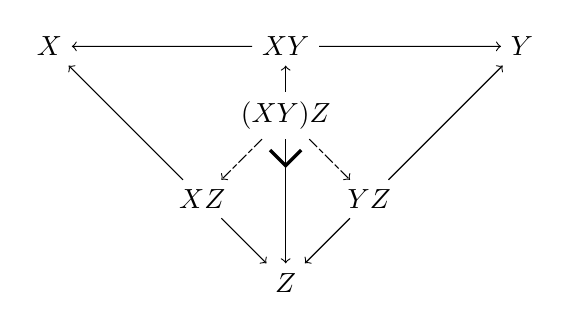
\begin{tikzpicture}[scale=3]
\node(X) at (-1, 1) {$X$};
\node(Y) at (1, 1) {$Y$};
\node(Z) at (0, 0) {$Z$};
\node(XY) at (0, 1) {$X \boxtimes Y$};
\node(XZ) at ({0.5*-sin(45)}, {0.5*cos(45)}) {$X \boxtimes Z$};
\node(YZ) at ({0.5*sin(45)}, {0.5*cos(45)}) {$Y \boxtimes Z$};
\node(XYZ) at (0, {0.5*2*cos(45)}) {$(X \boxtimes Y) \boxtimes Z$};
\path[->]
(XY) edge (X)
(XY) edge (Y)
(XZ) edge (X)
(XZ) edge (Z)
(YZ) edge (Y)
(YZ) edge (Z)
(XYZ) edge (XY)
(XYZ) edge (Z)
(XYZ) edge[dash pattern=on 4pt off 1pt on 2pt off 1pt] (XZ)
(XYZ) edge[dash pattern=on 4pt off 1pt on 2pt off 1pt] (YZ);
\draw[very thick] ({-(1-0.7)*0.5*2*cos(45)/2+0.04}, {0.5*2*cos(45)-(1-0.7)*0.5*2*cos(45)/2-0.04}) --
                  (0, {0.7*0.5*2*cos(45)}) --
                  ({ (1-0.7)*0.5*2*cos(45)/2-0.04}, {0.5*2*cos(45)-(1-0.7)*0.5*2*cos(45)/2-0.04});
\end{tikzpicture}
\noindent We again intend to view a pullback as a product of slices, and instantiate \autoref{prop:midpoint} in |SliceCategory Fam (I , μ D)|, substituting all the objects by slices consisting of relevant ornamental forgetful functions in~(\ref{eq:modularity}).
The substitutions are as follows:
\[ \begin{array}{rcl}
X                            & \mapsto & |slice _ (_ , forget O)| \\
Y                            & \mapsto & |slice _ (_ , forget P)| \\
X \boxtimes Y                & \mapsto & |slice _ (_ , forget ⌈ O ⊗ P ⌉)| \\
Z                            & \mapsto & |slice _ (_ , forget ⌈ S ⌉)| \\
X \boxtimes Z                & \mapsto & |slice _ (_ , forget ⌈ O ⊗ ⌈ S ⌉ ⌉)| \\
Y \boxtimes Z                & \mapsto & |slice _ (_ , forget ⌈ P ⊗ ⌈ S ⌉ ⌉)| \\
(X \boxtimes Y) \boxtimes Z  & \mapsto & |slice _ (_ , forget ⌈ ⌈ O ⊗ P ⌉ ⊗ ⌈ S ⌉ ⌉)|
\end{array} \]
where $X \boxtimes Y$, $X \boxtimes Z$, $Y \boxtimes Z$, and $(X \boxtimes Y) \boxtimes Z$ indeed give rise to products in |SliceCategory Fam (I , μ D)|, i.e., pullbacks in |Fam|, by instantiating \autoref{prop:pullback-Fam}.
What we get out of this instantiation of the lemma is a pullback in |SliceCategory Fam (I , μ D)| rather than |Fam|.
This is easy to fix, since there is a forgetful functor from any |SliceCategory C B| to~|C| whose object part is |Slice.T|, and it is pullback-preserving.
We thus get a pullback in |Fam| which is based on the same slices as~(\ref{eq:N-pullback}) and has vertex |(pull ⋈ proj₁ , M)|.

Having the two pullbacks, by \autoref{prop:pullback-iso} we get an isomorphism in |Fam| between |(pull ⋈ proj₁ , M)| and |(pull ⋈ proj₁ , N)|, whose index part can be shown to be identity, so there are componentwise isomorphisms between |M|~and~|N| in |Fun|, arriving at~(\ref{eq:modularity}).
